\documentclass[10pt]{book}
\usepackage[utf8]{inputenc}
\usepackage{geometry}
\usepackage{ngerman}
\usepackage[right]{eurosym}
\usepackage{titlesec}
\usepackage{graphicx}
\usepackage{caption}
\usepackage{flowfram}
\usepackage{tikz}
\usepackage{textpos}
\usepackage{calc}
\usepackage{amsmath, amssymb}
\usepackage{lastpage}
\usepackage{float}
\usepackage{ifthen}
\usepackage{changepage}
\usepackage{pgfplots}
\usepackage{sectsty}
\usepackage{tikz,xcolor,mwe}
\usepackage{booktabs,xcolor,siunitx}

\usetikzlibrary{arrows,
		calc,
		shadows,
		decorations.markings}

\definecolor{cvgreen}{HTML}{92D14F}
\definecolor{cvgray}{HTML}{D8E4BE}
\definecolor{cvtext}{HTML}{000000}
\definecolor{cvtabt}{HTML}{e5e2cc}

\definecolor{lightgray}{gray}{0.9}

\pgfplotsset{compat=1.9}

\setlength{\parindent}{0em} 

\newcommand\titelpage{%
\begin{tikzpicture}[overlay, remember picture]
    % green bar
    \fill[cvgreen] (current page.north west) rectangle ([xshift=5cm]current page.south west);
    % gray bar
    \fill[cvgray] ([yshift=-5cm]current page.north west) rectangle ([yshift=-10cm]current page.north east);
    % title and date
    \node[cvtext,right] at ([yshift=-7cm]current page.north west) {\Huge\bfseries Mathe-Notizen f"ur Selbstudium};
    \node[cvtext,right] at ([yshift=-8cm]current page.north west) {\Huge 1. Auflage};
    \node[cvtext,above left] at ([xshift=-1cm,yshift=-9.5cm]current page.north east) {\Huge\bfseries vom \today };
    % cover photo
    \node[inner sep=0pt,below right] (image) at ([xshift=5cm,yshift=-10cm]current page.north west)
    {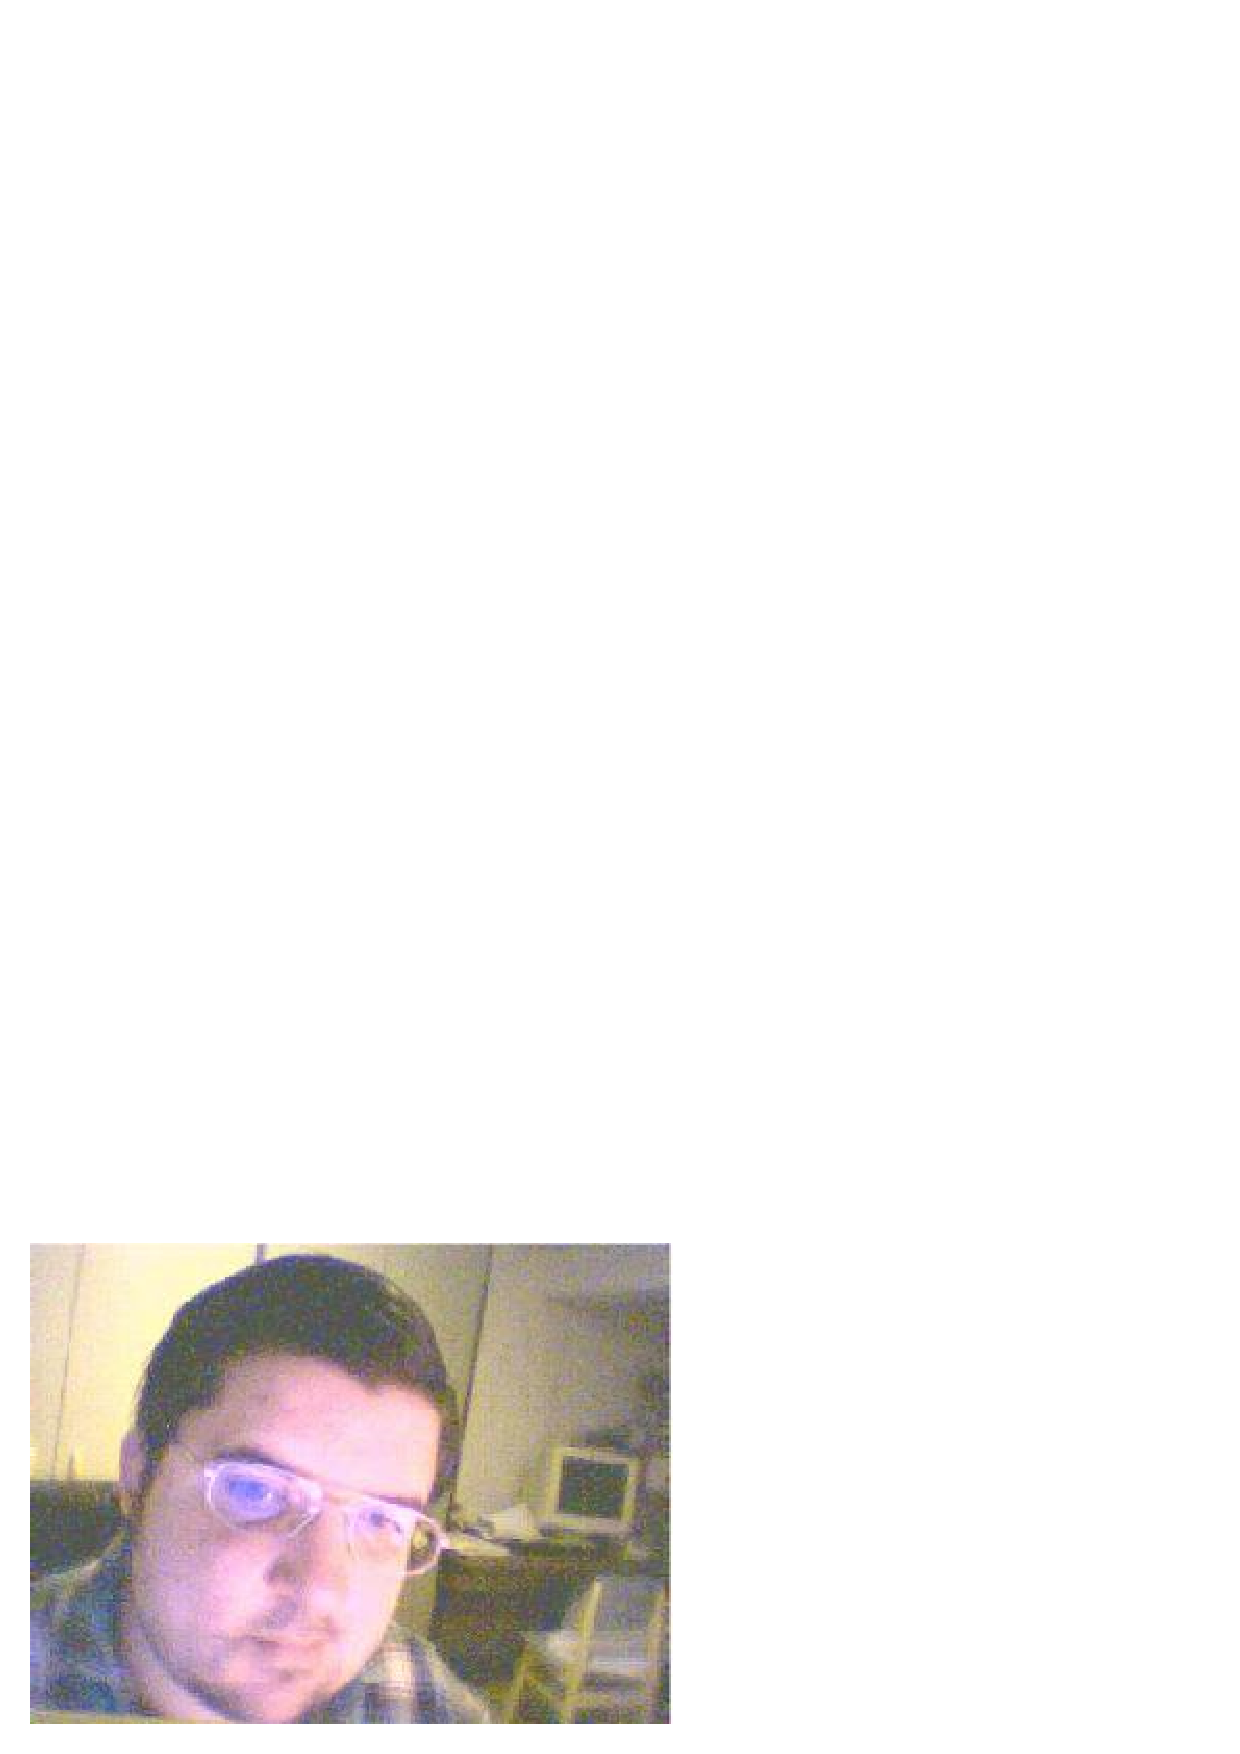
\includegraphics[width=11cm,height=9cm]{pics/me.jpg}};
    % name and address
    \node[fill=white,drop shadow,align=center,text width=6.4cm,inner sep=0.3cm,below] (name) at (image.south)
        {\LARGE Jens Kallup};
    \node[text width=15cm,inner sep=0.3cm,below right] at (name.south west) {\Large\obeylines%
        Langensalzer Str. 30\\
        99817 Eisenach\\
        Tel.: 03691 / \\
        E-Mail: jkallup@web.de
    };
    % attachments
    \node[black,text width=5cm,inner sep=0.3cm,above right] at ([yshift=1cm]current page.south west) {\large\obeylines%
        \textbf{Inhalt:}\\[4pt]
        Eigene Gedanken zu:\\[3pt]
        de.sci.mathematik \\
        de.sci.informatik
    };
\end{tikzpicture}}


\titleformat{name=\chapter}[display]{\Huge\bfseries\sffamily\color{white}}{%
\thispagestyle{empty}
\begin{tikzpicture}[overlay, remember picture]
        \path let \p1 = (current page.west), \p2 = (current page.east) in
        node[minimum width=\x2-1.5pt, minimum height=4cm,
        rectangle, fill=cyan, anchor=north west, align=left, text width=\x2-\x1] at ($(current page.north west)$) {
        \begin{textblock*}{5in}(\dimexpr\x2-4.0in,\dimexpr0.25\headheight-1in)
          \tikz \node [white,text width=2in, align=right, font=\sffamily] {{\normalsize MATHEMATIK }\\[10pt]
          \raisebox{20pt}{{\large \chaptertitlename}} \raisebox{-12pt}{\chapternumberfont \thechapter}};
        \end{textblock*}};
        \path let \p1 = (current page.west), \p2 = (current page.east) in
              node[minimum width=\x2-\x1, minimum height=-2.8in, rectangle, fill=cyan!50, anchor=south west, align=left, text width=\x2-\x1] at ($(current page.south west)$) {\textcolor{black}{\Large{\thepage . \: \: de.sci.mathematik}}};
\end{tikzpicture}}{-1.75in}{}[\vspace*{0.25in}]


\titleformat{name=\chapter,numberless}[display]{\Huge{\bfseries\sffamily\color{yellow}}}{%
   \thispagestyle{empty}
  \begin{tikzpicture}[overlay, remember picture]
     \path let \p1 = (current page.west), \p2 = (current page.east) in
     node[minimum width=\x2-1.5pt, minimum height=4cm,
     rectangle, fill=cyan, anchor=north west, align=left, text width=\x2-\x1] at ($(current page.north west)$) {
        \begin{textblock*}{5in}(\dimexpr\x2-4.0in,\dimexpr0.25\headheight-1in)
           \tikz \node [white,text width=2in, align=right, font=\sffamily] {{\normalsize MATHEMATIK }\\[10pt]
           \raisebox{20pt}{{\large \chaptertitlename}} \raisebox{-12pt}{\chapternumberfont \thechapter}};
     \end{textblock*}
  };
     \fill[cyan](current page.south west) rectangle ($(current page.south east) - (0,-1.5cm)$);
\end{tikzpicture}}{-1.75in}{}[\vspace*{0.25in}]
 
\titleformat{name=\section}[display]{\Huge{\bfseries\sffamily\color{yellow}}}{%
   \thispagestyle{empty}
  \begin{tikzpicture}[overlay, remember picture]
     \path let \p1 = (current page.west), \p2 = (current page.east) in
     node[minimum width=\x2-1.5pt, minimum height=4cm,
     rectangle, fill=cyan, anchor=north west, align=left, text width=\x2-\x1] at ($(current page.north west)$) {
        \begin{textblock*}{5in}(\dimexpr\x2-4.0in,\dimexpr0.25\headheight-1in)
           \tikz \node [white,text width=2in, align=right, font=\sffamily]
           {\normalsize MATHEMATIK }\\[10pt];
        \end{textblock*}
  };
     \fill[cyan](current page.south west) rectangle ($(current page.south east) - (0,-1.5cm)$);
\end{tikzpicture}}{-1.75in}{}[\vspace*{0.25in}]
 
\titleformat{name=\subsection}{\Huge{\bfseries\sffamily\color{yellow}}}{%
   \thispagestyle{empty}
  \begin{tikzpicture}[overlay, remember picture]
     \path let \p1 = (current page.west), \p2 = (current page.east) in
     node[minimum width=\x2-1.5pt, minimum height=4cm,
     rectangle, fill=cyan, anchor=north west, align=left, text width=\x2-\x1] at ($(current page.north west)$) {
        \begin{textblock*}{5in}(\dimexpr\x2-4.0in,\dimexpr0.25\headheight-1in)
           \tikz \node [white,text width=2in, align=right, font=\sffamily] {{\normalsize MATHEMATIK }\\[10pt]
           \raisebox{20pt}{{\large \chaptertitlename}} \raisebox{-12pt}{\chapternumberfont \thechapter}};
     \end{textblock*}};
     \fill[cyan](current page.south west) rectangle ($(current page.south east) - (0,-1.5cm)$);
\end{tikzpicture}}{-1.75in}{}[\vspace*{0.25in}]
 
\titleformat{name=\subsubsection}[display]{\Huge{\bfseries\sffamily\color{yellow}}}{%
   \thispagestyle{empty}
  \begin{tikzpicture}[overlay, remember picture]
     \path let \p1 = (current page.west), \p2 = (current page.east) in
     node[minimum width=\x2-1.5pt, minimum height=4cm,
     rectangle, fill=cyan, anchor=north west, align=left, text width=\x2-\x1] at ($(current page.north west)$) {
        \begin{textblock*}{5in}(\dimexpr\x2-4.0in,\dimexpr0.25\headheight-1in)
           \tikz \node [white,text width=2in, align=right, font=\sffamily] {{\normalsize MATHEMATIK }\\[10pt]
           \raisebox{20pt}{{\large \chaptertitlename}} \raisebox{-12pt}{\chapternumberfont \thechapter}};
     \end{textblock*}};
     \fill[cyan](current page.south west) rectangle ($(current page.south east) - (0,-1.5cm)$);
\end{tikzpicture}}{-1.75in}{}[\vspace*{0.25in}]





\newcommand*\MyHeadBottom{%
\makeatletter
\strictpagecheck
\ifoddpage\else
\thispagestyle{empty}
\begin{tikzpicture}[overlay, remember picture]
\checkoddpage
	\path let \p1 = (current page.west), \p2 = (current page.east) in
        node[minimum width=\x2-1.5pt, minimum height=2cm,
        rectangle, fill=cyan, anchor=north west, align=left, text width=\x2-\x1] at ($(current page.north west)$) {
        \begin{textblock*}{5in}(\dimexpr\x2-4.0in,\dimexpr0.25\headheight-1cm)
          \tikz \node [white,text width=2in, align=right, font=\sffamily] {{\normalsize Neuronale Netze }\\[10pt]
                    \raisebox{20pt}{{\large \chaptertitlename}} \raisebox{-10pt}{\chapternumberfont \thechapter}};
        \end{textblock*}};
	\path let \p1 = (current page.west), \p2 = (current page.east) in
	              node[minimum width=\x2-\x1, minimum height=1cm, rectangle, fill=cyan!50, anchor=south west, align=right, text width=\x2-\x1] at
	        ($(current page.south west)$) {\textcolor{black}{\Large{\textbf{de.sci.mathematik \: \thepage . \: \:}}}};
\end{tikzpicture}
\fi
\makeatother
}

\newenvironment{MyConsoleBox}[1]
%BEGIN
{%
  \begingroup\setlength{\textwidth}{20cm}
  \colorbox{lightgray}{%
  \begin{tabular}{p{14.4cm}}
  #1
  \end{tabular}
  }\endgroup
}%
%END
{%
}


\newenvironment{MyTableBox}[1]
%BEGIN
{%
  \begingroup\setlength{\textwidth}{20cm}
  \colorbox{cvtabt}{%
  \begin{tabular}{|p{4cm}|p{5cm}|p{4cm}|}
  \hline
  #1
  \hline
  \end{tabular}
  }\endgroup
}%
%END
{%
}

\newcommand\bildzrange{%
\begin{tikzpicture}[overlay, remember picture]
   \node[inner sep=0pt,below right] (image) at ([xshift=-10cm,yshift=-3.1cm]current page.north east)
  {\includegraphics[width=7.5cm,height=4.1cm]{pics/zbereiche.jpg}};
\end{tikzpicture}}

\newcommand\legendezbereiche{%
\begin{tabular}{ll}
 $\mathbb{C}$  & = komplexe Zahl    \\
 $\mathbb{I}$  & = irrationale Zahl \\
 $\mathbb{N}$  & = natürliche Zahl  \\
 $\mathbb{Q}$  & = rationale Zahl   \\
 $\mathbb{R}$  & = reelle Zahl      \\
 $\mathbb{Z}$  & = ganze Zahl       \\
\end{tabular}
\\
\begin{tabular}{ll}
 $ f $         & = Funktion \\
 $ x $         & = Argument, x-Wert, unabhängige Variable  \\
 $ y $         & = Funktionswert, y-Wert, abhängige Variable  \\
 $ y = f(x) $  & = Funktionsgleichung, Zuordnungsvorschrift  \\
 $ f(x) $      & = spricht man ''f von x'' \\
 $ D \: (oder \: \mathbb{D} ) $ & = Definitionsmenge, Definitionsbereich  \\
 $ W $         & = Wertemenge, Wertebereich \\
 & \\
 $ f(x) = c $  & = konstante Funktion \\
 $ f(x) = mx + n $ & = lineare Funktion \\
 $ f(x) = ax^2 + bx + c $ & = quadratische Funktion \\
 $ f(x) = \frac{a_n x^a_n + a_n -1^{x^{n-1}} + \ldots + a_1 x + a_0}{a_m x^m + b_m -1^{x^{m-1}} + \ldots + b_1 x + b_0} $ &
 = rationale gebrochene Funktion
\end{tabular}}


  
\begin{document}
\titelpage
\tableofcontents
\listoftables
\listoffigures

\chapter{Vorwort}
mit diesen Posting will ich versuchen, eine Zusammenfassung
dessen zu geben, was hier seit Monaten Diskutiert wird.
Falls was falsch sein sollte, bitte Feedback geben.
Kann auch passieren das ich aus versehen eine falsche Taste
beim schreiben drücke, und der Inhalt fehlt, ich bemühe mich
durchgängig zu schreiben und im Zusammenhang zu posten.
Ok, let's go...



\chapter{Mathe - Klasse 1}
\pagestyle{empty}
\section{Übungen 1}
Rechne aus: \\ \\
\begin{minipage}{\textwidth}
\begin{tabular}{p{1cm}p{1cm}p{1cm}p{1cm}p{1cm}}
  \begin{tikzpicture}
    \shade[ball color=green] (9,0.5) circle (0.5cm); 
  \end{tikzpicture} &
  \begin{tikzpicture}
    \shade[ball color=green] (9,0.5) circle (0.5cm);
  \end{tikzpicture} &
  \begin{tikzpicture}
    \shade[ball color=green] (9,0.5) circle (0.5cm);
  \end{tikzpicture}
\end{tabular}

\begin{tabular}{p{1cm}p{1cm}p{1cm}p{1cm}p{1cm}}
  &
  \begin{tikzpicture}
    \shade[ball color=green] (2,-1.5) circle (0.5cm); 
  \end{tikzpicture}
\end{tabular}

\vspace{1.0cm}
\begin{tikzpicture}
\draw ( 0, 1.5) -- (-4 , 1.5);
\end{tikzpicture}
\vspace{1.0cm}

\begin{tabular}{p{1cm}p{1cm}p{1cm}p{1cm}p{1cm}}
  \begin{tikzpicture}
    \shade[ball color=green] (9,0.5) circle (0.5cm); 
  \end{tikzpicture} &
  \begin{tikzpicture}
    \shade[ball color=green] (9,0.5) circle (0.5cm);
  \end{tikzpicture} &
  \begin{tikzpicture}
    \shade[ball color=green] (9,0.5) circle (0.5cm); 
  \end{tikzpicture}
\end{tabular}

\vspace{1.25cm}
\begin{tikzpicture}
\draw ( 0, 1.5) -- (-4 , 1.5);
\end{tikzpicture}
\vspace{1.0cm}


\hspace{0.75cm}
\begin{tabular}{p{1.0cm}p{1.0cm}}
  \begin{tikzpicture}
    \shade[ball color=green] (9,0.5) circle (0.5cm);
  \end{tikzpicture} &
  \begin{tikzpicture}
    \shade[ball color=green] (9,0.5) circle (0.5cm); 
  \end{tikzpicture}
\end{tabular}

\vspace{1.0cm}
\begin{tikzpicture}
\draw ( 0, 1.5) -- (-4 , 1.5);
\end{tikzpicture}

\vspace{1.0cm}
\hspace{0.75cm}
\begin{tabular}{p{1.0cm}p{1.0cm}}
  \begin{tikzpicture}
    \shade[ball color=green] (9,0.5) circle (0.5cm);
  \end{tikzpicture} &
  \begin{tikzpicture}
    \shade[ball color=green] (9,0.5) circle (0.5cm); 
  \end{tikzpicture}
\end{tabular}

\vspace{1.0cm}
\begin{tikzpicture}
\draw ( 0, 1.5) -- (-4 , 1.5);
\end{tikzpicture}

\vspace{1.0cm}
\hspace{1.50cm}
\begin{tabular}{p{1.0cm}}
  \begin{tikzpicture}
    \shade[ball color=green] (9,0.5) circle (0.5cm); 
  \end{tikzpicture}
\end{tabular}

\vspace{1cm}
\begin{tikzpicture}
\draw ( 0, 0) -- (-4 , 0);
\end{tikzpicture}
\end{minipage}

\chapter{Mathe - Klasse 1}
\section{Übungen 2}
Rechne aus: \\ \\
\begin{tabular}{p{3cm}p{3cm}p{3cm}p{3cm}p{3cm}}
\begin{tikzpicture}
% Figur-Körper
\draw ( 0, 0 ) -- ( 1,  1 );
\draw ( 2, 0 ) -- ( 0,  0 );
\draw ( 2, 0 ) -- ( 1,  1 );
\draw ( 2, 0 ) -- ( 2, -2.5 );
\draw ( 0, 0 ) -- ( 0, -2.5 );

\draw ( 0, -0.5) -- ( 2, -0.5 );
\draw ( 0, -1.0) -- ( 2, -1.0 );
\draw ( 0, -1.5) -- ( 2, -1.5 );
\draw ( 0, -2.0) -- ( 2, -2.0 );
\draw ( 0, -2.5) -- ( 2, -2.5 );

% Teiler (r/l)
\draw ( 1, -2.5) -- ( 1, 0 );
\draw ( 1, 0.32) node { + 7 };

\draw ( 0.5, -0.25 ) node { 20 };
\draw ( 0.5, -0.75 ) node {  8 };
\draw ( 0.5, -1.25 ) node { 15 };
\draw ( 0.5, -1.75 ) node { 12 };
\draw ( 0.5, -2.25 ) node {  9 };
\end{tikzpicture}

&

\begin{tikzpicture}
\draw ( 0, 0 ) -- ( 1,  1 );
\draw ( 2, 0 ) -- ( 0,  0 );
\draw ( 2, 0 ) -- ( 1,  1 );
\draw ( 2, 0 ) -- ( 2, -2.5 );
\draw ( 0, 0 ) -- ( 0, -2.5 );

\draw ( 0, -0.5) -- ( 2, -0.5 );
\draw ( 0, -1.0) -- ( 2, -1.0 );
\draw ( 0, -1.5) -- ( 2, -1.5 );
\draw ( 0, -2.0) -- ( 2, -2.0 );
\draw ( 0, -2.5) -- ( 2, -2.5 );

% Teiler (r/l)
\draw ( 1, -2.5) -- ( 1, 0 );
\draw ( 1, 0.32) node { + 7 };

\draw ( 0.5, -0.25 ) node { 20 };
\draw ( 0.5, -0.75 ) node {  8 };
\draw ( 0.5, -1.25 ) node { 15 };
\draw ( 0.5, -1.75 ) node { 12 };
\draw ( 0.5, -2.25 ) node {  9 };

\end{tikzpicture}

&

\begin{tikzpicture}
\draw ( 0, 0 ) -- ( 1,  1 );
\draw ( 2, 0 ) -- ( 0,  0 );
\draw ( 2, 0 ) -- ( 1,  1 );
\draw ( 2, 0 ) -- ( 2, -2.5 );
\draw ( 0, 0 ) -- ( 0, -2.5 );

\draw ( 0, -0.5) -- ( 2, -0.5 );
\draw ( 0, -1.0) -- ( 2, -1.0 );
\draw ( 0, -1.5) -- ( 2, -1.5 );
\draw ( 0, -2.0) -- ( 2, -2.0 );
\draw ( 0, -2.5) -- ( 2, -2.5 );

% Teiler (r/l)
\draw ( 1, -2.5) -- ( 1, 0 );
\draw ( 1, 0.32) node { + 7 };

\draw ( 0.5, -0.25 ) node { 20 };
\draw ( 0.5, -0.75 ) node {  8 };
\draw ( 0.5, -1.25 ) node { 15 };
\draw ( 0.5, -1.75 ) node { 12 };
\draw ( 0.5, -2.25 ) node {  9 };

\end{tikzpicture}

&

\begin{tikzpicture}
\draw ( 0, 0 ) -- ( 1,  1 );
\draw ( 2, 0 ) -- ( 0,  0 );
\draw ( 2, 0 ) -- ( 1,  1 );
\draw ( 2, 0 ) -- ( 2, -2.5 );
\draw ( 0, 0 ) -- ( 0, -2.5 );

\draw ( 0, -0.5) -- ( 2, -0.5 );
\draw ( 0, -1.0) -- ( 2, -1.0 );
\draw ( 0, -1.5) -- ( 2, -1.5 );
\draw ( 0, -2.0) -- ( 2, -2.0 );
\draw ( 0, -2.5) -- ( 2, -2.5 );

% Teiler (r/l)
\draw ( 1, -2.5) -- ( 1, 0 );
\draw ( 1, 0.32) node { + 7 };

\draw ( 0.5, -0.25 ) node { 20 };
\draw ( 0.5, -0.75 ) node {  8 };
\draw ( 0.5, -1.25 ) node { 15 };
\draw ( 0.5, -1.75 ) node { 12 };
\draw ( 0.5, -2.25 ) node {  9 };

\end{tikzpicture}

&

\begin{tikzpicture}
\draw ( 0, 0 ) -- ( 1,  1 );
\draw ( 2, 0 ) -- ( 0,  0 );
\draw ( 2, 0 ) -- ( 1,  1 );
\draw ( 2, 0 ) -- ( 2, -2.5 );
\draw ( 0, 0 ) -- ( 0, -2.5 );

\draw ( 0, -0.5) -- ( 2, -0.5 );
\draw ( 0, -1.0) -- ( 2, -1.0 );
\draw ( 0, -1.5) -- ( 2, -1.5 );
\draw ( 0, -2.0) -- ( 2, -2.0 );
\draw ( 0, -2.5) -- ( 2, -2.5 );

% Teiler (r/l)
\draw ( 1, -2.5) -- ( 1, 0 );
\draw ( 1, 0.32) node { + 7 };

\draw ( 0.5, -0.25 ) node { 20 };
\draw ( 0.5, -0.75 ) node {  8 };
\draw ( 0.5, -1.25 ) node { 15 };
\draw ( 0.5, -1.75 ) node { 12 };
\draw ( 0.5, -2.25 ) node {  9 };

\end{tikzpicture}
\end{tabular}

\vspace{2cm}
%--------------------------

\begin{tabular}{p{3cm}p{3cm}p{3cm}p{3cm}p{3cm}}
\begin{tikzpicture}
% Figur-Körper
\draw ( 0, 0 ) -- ( 1,  1 );
\draw ( 2, 0 ) -- ( 0,  0 );
\draw ( 2, 0 ) -- ( 1,  1 );
\draw ( 2, 0 ) -- ( 2, -2.5 );
\draw ( 0, 0 ) -- ( 0, -2.5 );

\draw ( 0, -0.5) -- ( 2, -0.5 );
\draw ( 0, -1.0) -- ( 2, -1.0 );
\draw ( 0, -1.5) -- ( 2, -1.5 );
\draw ( 0, -2.0) -- ( 2, -2.0 );
\draw ( 0, -2.5) -- ( 2, -2.5 );

% Teiler (r/l)
\draw ( 1, -2.5) -- ( 1, 0 );
\draw ( 1, 0.32) node { + 7 };

\draw ( 0.5, -0.25 ) node { 20 };
\draw ( 0.5, -0.75 ) node {  8 };
\draw ( 0.5, -1.25 ) node { 15 };
\draw ( 0.5, -1.75 ) node { 12 };
\draw ( 0.5, -2.25 ) node {  9 };
\end{tikzpicture}

&

\begin{tikzpicture}
\draw ( 0, 0 ) -- ( 1,  1 );
\draw ( 2, 0 ) -- ( 0,  0 );
\draw ( 2, 0 ) -- ( 1,  1 );
\draw ( 2, 0 ) -- ( 2, -2.5 );
\draw ( 0, 0 ) -- ( 0, -2.5 );

\draw ( 0, -0.5) -- ( 2, -0.5 );
\draw ( 0, -1.0) -- ( 2, -1.0 );
\draw ( 0, -1.5) -- ( 2, -1.5 );
\draw ( 0, -2.0) -- ( 2, -2.0 );
\draw ( 0, -2.5) -- ( 2, -2.5 );

% Teiler (r/l)
\draw ( 1, -2.5) -- ( 1, 0 );
\draw ( 1, 0.32) node { + 7 };

\draw ( 0.5, -0.25 ) node { 20 };
\draw ( 0.5, -0.75 ) node {  8 };
\draw ( 0.5, -1.25 ) node { 15 };
\draw ( 0.5, -1.75 ) node { 12 };
\draw ( 0.5, -2.25 ) node {  9 };

\end{tikzpicture}

&

\begin{tikzpicture}
\draw ( 0, 0 ) -- ( 1,  1 );
\draw ( 2, 0 ) -- ( 0,  0 );
\draw ( 2, 0 ) -- ( 1,  1 );
\draw ( 2, 0 ) -- ( 2, -2.5 );
\draw ( 0, 0 ) -- ( 0, -2.5 );

\draw ( 0, -0.5) -- ( 2, -0.5 );
\draw ( 0, -1.0) -- ( 2, -1.0 );
\draw ( 0, -1.5) -- ( 2, -1.5 );
\draw ( 0, -2.0) -- ( 2, -2.0 );
\draw ( 0, -2.5) -- ( 2, -2.5 );

% Teiler (r/l)
\draw ( 1, -2.5) -- ( 1, 0 );
\draw ( 1, 0.32) node { + 7 };

\draw ( 0.5, -0.25 ) node { 20 };
\draw ( 0.5, -0.75 ) node {  8 };
\draw ( 0.5, -1.25 ) node { 15 };
\draw ( 0.5, -1.75 ) node { 12 };
\draw ( 0.5, -2.25 ) node {  9 };

\end{tikzpicture}

&

\begin{tikzpicture}
\draw ( 0, 0 ) -- ( 1,  1 );
\draw ( 2, 0 ) -- ( 0,  0 );
\draw ( 2, 0 ) -- ( 1,  1 );
\draw ( 2, 0 ) -- ( 2, -2.5 );
\draw ( 0, 0 ) -- ( 0, -2.5 );

\draw ( 0, -0.5) -- ( 2, -0.5 );
\draw ( 0, -1.0) -- ( 2, -1.0 );
\draw ( 0, -1.5) -- ( 2, -1.5 );
\draw ( 0, -2.0) -- ( 2, -2.0 );
\draw ( 0, -2.5) -- ( 2, -2.5 );

% Teiler (r/l)
\draw ( 1, -2.5) -- ( 1, 0 );
\draw ( 1, 0.32) node { + 7 };

\draw ( 0.5, -0.25 ) node { 20 };
\draw ( 0.5, -0.75 ) node {  8 };
\draw ( 0.5, -1.25 ) node { 15 };
\draw ( 0.5, -1.75 ) node { 12 };
\draw ( 0.5, -2.25 ) node {  9 };

\end{tikzpicture}

&

\begin{tikzpicture}
\draw ( 0, 0 ) -- ( 1,  1 );
\draw ( 2, 0 ) -- ( 0,  0 );
\draw ( 2, 0 ) -- ( 1,  1 );
\draw ( 2, 0 ) -- ( 2, -2.5 );
\draw ( 0, 0 ) -- ( 0, -2.5 );

\draw ( 0, -0.5) -- ( 2, -0.5 );
\draw ( 0, -1.0) -- ( 2, -1.0 );
\draw ( 0, -1.5) -- ( 2, -1.5 );
\draw ( 0, -2.0) -- ( 2, -2.0 );
\draw ( 0, -2.5) -- ( 2, -2.5 );

% Teiler (r/l)
\draw ( 1, -2.5) -- ( 1, 0 );
\draw ( 1, 0.32) node { + 7 };

\draw ( 0.5, -0.25 ) node { 20 };
\draw ( 0.5, -0.75 ) node {  8 };
\draw ( 0.5, -1.25 ) node { 15 };
\draw ( 0.5, -1.75 ) node { 12 };
\draw ( 0.5, -2.25 ) node {  9 };

\end{tikzpicture}
\end{tabular}

\vspace{2cm}
%--------------------------

\begin{tabular}{p{3cm}p{3cm}p{3cm}p{3cm}p{3cm}}
\begin{tikzpicture}
% Figur-Körper
\draw ( 0, 0 ) -- ( 1,  1 );
\draw ( 2, 0 ) -- ( 0,  0 );
\draw ( 2, 0 ) -- ( 1,  1 );
\draw ( 2, 0 ) -- ( 2, -2.5 );
\draw ( 0, 0 ) -- ( 0, -2.5 );

\draw ( 0, -0.5) -- ( 2, -0.5 );
\draw ( 0, -1.0) -- ( 2, -1.0 );
\draw ( 0, -1.5) -- ( 2, -1.5 );
\draw ( 0, -2.0) -- ( 2, -2.0 );
\draw ( 0, -2.5) -- ( 2, -2.5 );

% Teiler (r/l)
\draw ( 1, -2.5) -- ( 1, 0 );
\draw ( 1, 0.32) node { + 7 };

\draw ( 0.5, -0.25 ) node { 20 };
\draw ( 0.5, -0.75 ) node {  8 };
\draw ( 0.5, -1.25 ) node { 15 };
\draw ( 0.5, -1.75 ) node { 12 };
\draw ( 0.5, -2.25 ) node {  9 };
\end{tikzpicture}

&

\begin{tikzpicture}
\draw ( 0, 0 ) -- ( 1,  1 );
\draw ( 2, 0 ) -- ( 0,  0 );
\draw ( 2, 0 ) -- ( 1,  1 );
\draw ( 2, 0 ) -- ( 2, -2.5 );
\draw ( 0, 0 ) -- ( 0, -2.5 );

\draw ( 0, -0.5) -- ( 2, -0.5 );
\draw ( 0, -1.0) -- ( 2, -1.0 );
\draw ( 0, -1.5) -- ( 2, -1.5 );
\draw ( 0, -2.0) -- ( 2, -2.0 );
\draw ( 0, -2.5) -- ( 2, -2.5 );

% Teiler (r/l)
\draw ( 1, -2.5) -- ( 1, 0 );
\draw ( 1, 0.32) node { + 7 };

\draw ( 0.5, -0.25 ) node { 20 };
\draw ( 0.5, -0.75 ) node {  8 };
\draw ( 0.5, -1.25 ) node { 15 };
\draw ( 0.5, -1.75 ) node { 12 };
\draw ( 0.5, -2.25 ) node {  9 };

\end{tikzpicture}

&

\begin{tikzpicture}
\draw ( 0, 0 ) -- ( 1,  1 );
\draw ( 2, 0 ) -- ( 0,  0 );
\draw ( 2, 0 ) -- ( 1,  1 );
\draw ( 2, 0 ) -- ( 2, -2.5 );
\draw ( 0, 0 ) -- ( 0, -2.5 );

\draw ( 0, -0.5) -- ( 2, -0.5 );
\draw ( 0, -1.0) -- ( 2, -1.0 );
\draw ( 0, -1.5) -- ( 2, -1.5 );
\draw ( 0, -2.0) -- ( 2, -2.0 );
\draw ( 0, -2.5) -- ( 2, -2.5 );

% Teiler (r/l)
\draw ( 1, -2.5) -- ( 1, 0 );
\draw ( 1, 0.32) node { + 7 };

\draw ( 0.5, -0.25 ) node { 20 };
\draw ( 0.5, -0.75 ) node {  8 };
\draw ( 0.5, -1.25 ) node { 15 };
\draw ( 0.5, -1.75 ) node { 12 };
\draw ( 0.5, -2.25 ) node {  9 };

\end{tikzpicture}

&

\begin{tikzpicture}
\draw ( 0, 0 ) -- ( 1,  1 );
\draw ( 2, 0 ) -- ( 0,  0 );
\draw ( 2, 0 ) -- ( 1,  1 );
\draw ( 2, 0 ) -- ( 2, -2.5 );
\draw ( 0, 0 ) -- ( 0, -2.5 );

\draw ( 0, -0.5) -- ( 2, -0.5 );
\draw ( 0, -1.0) -- ( 2, -1.0 );
\draw ( 0, -1.5) -- ( 2, -1.5 );
\draw ( 0, -2.0) -- ( 2, -2.0 );
\draw ( 0, -2.5) -- ( 2, -2.5 );

% Teiler (r/l)
\draw ( 1, -2.5) -- ( 1, 0 );
\draw ( 1, 0.32) node { + 7 };

\draw ( 0.5, -0.25 ) node { 20 };
\draw ( 0.5, -0.75 ) node {  8 };
\draw ( 0.5, -1.25 ) node { 15 };
\draw ( 0.5, -1.75 ) node { 12 };
\draw ( 0.5, -2.25 ) node {  9 };

\end{tikzpicture}

&

\begin{tikzpicture}
\draw ( 0, 0 ) -- ( 1,  1 );
\draw ( 2, 0 ) -- ( 0,  0 );
\draw ( 2, 0 ) -- ( 1,  1 );
\draw ( 2, 0 ) -- ( 2, -2.5 );
\draw ( 0, 0 ) -- ( 0, -2.5 );

\draw ( 0, -0.5) -- ( 2, -0.5 );
\draw ( 0, -1.0) -- ( 2, -1.0 );
\draw ( 0, -1.5) -- ( 2, -1.5 );
\draw ( 0, -2.0) -- ( 2, -2.0 );
\draw ( 0, -2.5) -- ( 2, -2.5 );

% Teiler (r/l)
\draw ( 1, -2.5) -- ( 1, 0 );
\draw ( 1, 0.32) node { + 7 };

\draw ( 0.5, -0.25 ) node { 20 };
\draw ( 0.5, -0.75 ) node {  8 };
\draw ( 0.5, -1.25 ) node { 15 };
\draw ( 0.5, -1.75 ) node { 12 };
\draw ( 0.5, -2.25 ) node {  9 };

\end{tikzpicture}
\end{tabular}


\chapter{Grundlagen - Informatik}
\section{Grundlagen}
Die zum Erledigen einer Aufgabe erforderlichen Arbeitsschritte
lassen einen immer wiederkehrenden Rhytmus erkennen: \\
\textbf{E} - ingabe \\
\textbf{V} - erarbeitung \\
\textbf{A} - usgabe . \\
\\
Der Aufbau der Zentraleinheit aus elektronischen Schaltungen bringt
es mit sich, dass zur Datendarstellung nur zwei Zust"ande gegeben sind. \\
''Ja'' - Strom flie"sst und \\
''Nein'' - kein Strom. \\
Diese beiden Zust"ande werden mit \textbf{1} oder \textbf{0} bezeichnet.\\
Das Bit ist ein Bin"arzeichen, das die Zust"ande 1 und 0 annehmen kann.
Es ist zugleich die kleinste Informationseinheit, die Computer verstehen.
Alle Informationen m"ussen auf dem Bit aufgebaut werden.
\\
\\
Hinweis: F"ur Grundlagen der in der Inforamtik verwendeten Zahlensysteme,
finden Sie auch im Kapitel \ref{Mathegrundlagen} - \ref{Zahlensysteme}
auf Seite \pageref{Zahlensysteme} .


\chapter{Grundlagen - Mathematik}\label{Mathegrundlagen}
\section{Zahlensysteme}\label{Zahlensysteme}
In jedem Zahlensystem wird der Wert einer Ziffer durch ihre Stellung
innerhalb einer Zahl bestimmt. Die Grundlage eines jedem Zahlensystems ist
seine Basis.
\\
\begin{minipage}{1.5\textwidth}
\begin{tabular}{lrlcl}
Beispiel:  & m * $b^n$    & m     & = & Ziffernwert \\
           &              & b     & = & Basis \\
           &              & n     & = & Exponent \\
           &              & $b^n$ & = & Zahlenbasis \\
           &              &       &   & \\
           & $36_{(10)}$  &       &   & Zahlenbasis : 10 \\
\end{tabular}
\end{minipage}
\\
Zehner und Einer benennen den Stellenwert.\\
W"ahlt man dagegen einen andere Zahlenbasis, so "andert sich der Wert betr"achtlich.\\
\begin{minipage}{1.5\textwidth}
\begin{tabular}{lrlcrr}
           & $36_{(10)}$  &       &   &   Zahlenbasis : 16 & \\
Das egibt: &              &       &   &   $3 * 16^1$ =     & 48 \\
           &              &       &   & + $6 * 16^0$ =     &  6 \\
           &              &       &   & = $6 * 16^0$ =     & 54 \\
\end{tabular}
\end{minipage}

\subsection{Dualsystem}
Das duale System entspricht dem bin"aren Aufbau der elektronischen Datenverarbeitunh.
Es beruht auf der Basis 2 und ben"otigt nur die Ziffern 0 und 1.\\

\begin{minipage}{0.5\textwidth}
\begin{tabular}{llcr}
Beispiel:  & $10_{(2)}$ & = & $1 * 2^1$ = 2 \\
           &            & + & $0 * 2^0$ = 0 \\
           &            &   &           = 2 \\
\end{tabular}
\end{minipage}

\section{Umwandlung Dezimal - Dual}
Im ersten Fall wird die Dezimalzahl so lange durch die Basis 2 geteilt, bis das
Ergebnis Null erreicht ist. Die Reste der einzelnen Divisionen ergeben die
Dualzahl. Im zweiten Fall werden die Ziffernwerte mit den Stellenwerten der
Dualzahl multipliziert. Die Summe der Produkte ergibt die Dezimalzahl.
\\
\subsection{Dezimal nach Dual umwandeln}
\begin{minipage}{0.5\textwidth}
\begin{tabular}{rcrr}
29 : 2 & = & 14 + Rest 1 & \\
14 : 2 & = &  7 + Rest 0 & \\
 7 : 2 & = &  3 + Rest 1 & \\
 3 : 2 & = &  1 + Rest 1 & \\
 1 : 2 & = &  0 + Rest 1 &  =  $11101_{(2)}$ \\
\end{tabular}
\end{minipage}
\\
\subsection{Dual in Dezimalzahl umwandeln}
\begin{minipage}{0.5\textwidth}
\begin{tabular}{lrrcrl}
1 1 1 0 1 & = 1 * &  1 & = &  1 & \\
          &   0 * &  0 & = &  0 & \\
          &   1 * &  4 & = &  4 & \\
          &   1 * &  8 & = &  8 & \\
          &   1 * & 16 & = & 16 &  = $29_{(10)}$ \\
\end{tabular}
\end{minipage}

\section{Hexadezimalsystem}
In diesem System liegt die Basis 16 zu Grunde, d. h. es werden 16 Ziffern ben"otigt.
Die ersten zehn Ziffern entstammen dem Dezimalsystem, 0 bis 9, die folgenden sechs
Ziffern werden beginnend mit den ersten Buchstaben des Alphabets bezeichnet, also A bis F. \\

\begin{minipage}{0.5\textwidth}
\begin{tabular}{lcccccccccccccccc}
dual: & 0 & 1 & 2 & 3 & 4 & 5 & 6 & 7 & 8 & 9 & 10 & 11 & 12 & 13 & 14 & 15 \\
hex:  & 0 & 1 & 2 & 3 & 4 & 5 & 6 & 7 & 8 & 9 & A  & B  & C  & D  & E  & F
\end{tabular}
\end{minipage}

\subsection{Umwandlung Hex nach Dezimal}
Folgende Hexadezimalzahl ist gegeben: 2AE\\
\\
\begin{minipage}{0.5\textwidth}
\begin{tabular}{lcrccrrl}
2 & = &  2 & * & $16^2$ & = & $512_{(10)}$ \\
A & = & 10 & * & $16^1$ & = & $160_{(10)}$ \\
E & = & 14 & * & $16^0$ & = & $ 14_{(10)}$ &  = $686_{(10)}$ \\
\end{tabular}
\end{minipage}

\section{Zeichen und Symbole}

\begin{minipage}{0.5\textwidth}
    \centering
    \captionof{figure}{Test figure}
    \legendezbereiche \bildzrange
    \label{fig:zahlenbereiche}
\end{minipage}


\chapter{Zahlen und Zahlenbereiche}
\section{Nat"urliche Zahlen}
\subsection{Einf"uhrung}
Der Begriff Zahl ist vom althochdeutschen Wort ''zala'' abgeleitet.
Dieser Begriff wurde mit ''Einschnitt ins Kerbholz'' "ubersetzt.
Diese "Ubersetzung zeigt, welche Bedeutung der Zahlbegriff historisch hatte.
Er sollte helfen, die Welt messbar und z"ahlbar zu machen. Die V"olker mit einer
schriftlichen Kultur haben im Laufe der Geschichte verschiedene Zahlen- und Notationsysteme
entwickelt. \\
Unser heutiges Zahlensystem wird arabisch-indisches System genannt. Es basiert auf
dem Dezimalsystem und enth"alt die Ziffern 0 bis 9. Aus diesen Symbolen oder Zeichen lassen
sich nach einfachen Gesetzm"assigkeiten beliebige Zahlen bilden.
Die beiden Begriffe Kardinalzahlen und Ordinalzahlen beschreiben jeweils die T"atigket des
Ordnens und des Z"ahlens.
Unter Kardinalzahlen versteht man die ganzen Zahlen, mit denen gez"ahlt wird und Mengen
beschrieben werden. Beispielsweise spricht man von 2 Hunden, 4 Katzen, 32 Kilometer usw.
Die Ordinalzahlen hingegen beschreiben Ordnungen, Rang- und Reihenfolgen.
Jemand gewinnt den 2. Preis oder schaut zum 10ten Mal 425 Folge von BibBangTheory.\\
\\
Nat"urliche Zahlen $N$ sind \textbf{positive} Zahlen, die durch 0
bis 9 symbolisiert dargestellt werden.
Nat"urliche Zahlen k"onnen gepaart werden, indem man an den Zahlen 1 bis 9
weitere natürliche Zahlen anf"ugt (zum Bsp.: 12, 34, 22).
Bei der Aufstellung der nat"urlichen Zahlen ist wie in der mathelogie
"ublich eine einheitliche Form einzuhalten.
So kann/darf man bei einer Definition nicht einfach: 12, 1 33
schreiben !!! \\
Es ist zwar keine feste Regel daf"ur manifestiert, aber der "Ubersichtlichkeit
ist eine gewisse Disziplin der Ordnung nicht falsch. \\
\\
Die Menge der nat"urlichen \textbf{positiven} Zahlen werden wie folgt
definiert: \\
$N = \{ 0;1;2;3; \ldots \}$ \\
\\
Nat"urliche Zahlen sind nur innerhalb eines mehr oder weniger
gro"sen Bereichs abz"ahlbar, da sie unendlich sind. Jede nat"urliche Zahl
\textbf{n} hat immer einen unmittelbaren Nachfolger \textbf{n + 1} hat.

\section{ganze Zahlen}
\subsection{Einf"uhrung}
Das Ergebnis einer Addition oder einer Multiplikation zweier nat"urlicher Zahlen
is immer eine weitere nat"urliche Zahl. Man sagt, dass die Menge der n"urllichen Zahlen
bez"uglich der Addition und der Multiplikation in sich abgeschlossen sind.
Achtung: Dies gilt nicht für die Subtraktion und der Division !\\
Die Subtraktion zweier nat"urlichen Zahlen ist nur mit den im na"urlichen Wertebereich
der Zahlen 0 bis 9 möglich \textbf{und} wenn der Minuend größer ist als der Subtrahend.
Ist jedoch der Minuend größer als der Subtrahend, ist das Ergebnis der Subtraktion keine
nat"urliche Zahl mehr. Deshalb werden die nat"urlichen Zahlen um die negativen Zahlem
erg"angzt.\\
Ganze Zahlen $Z$ erweitern die nat"urlichen Zahlen $N$.

\section{rationale Zahlen}
\subsection{Einf"uhrung}
Die Menge der nat"urlichen Zahlen ist abgeschlossen bez"uglich der Addition und Multiplikation,
nicht jedoch bez"uglich der Subtraktion und Divison. Deshalb wurden die nat"urlichen Zahlen zu
den ganzen Zahlen erweitert. Die Menge der ganzen Zahlen ist nun auch abgeschlossen. Allerdings
ist die Division in den ganzen Zahlen nicht uneingeschr"ankt m"oglich.\\
Deshalb wird der Zahlenbereich nun ein zweites Mal erweitert, so dass er auch abgeschlossen ist.
Die neu einzuf"uhrenden Zahlen sind die Brüche, die als:\\
$\frac{a}{b}$ \\
geschrieben werden.

\section{gebrochene Zahlen}
\subsection{Einf"uhrung}
Gebrochene Zahlen $Q+$ oder $Q*$ sind eine Erweiterung der nat"urlichen
Zahlen $N$, die gestattet, uneingeschränkt zu dividieren.
Dazu werden nat"urliche Zahlen um den \textbf{negativen} Zahlenbereich von
$N$ sowie um Br"uche (rationale Zahlen $Q$) erg"anzt.\\
\\
Addition und Maltiplikation k"onnen als ''abgeschlossene Operationen'' betrachtet werden.
Die Summe zweier nat"urlicher Zahlen ergibt immer eine weitere nat"urliche Zahl:
\\
$3 + 5 = 8 \:\:\:\:\:\:\: | \:\: 3 \in \mathbb{N}; \: 5 \in \mathbb{N}; \: 8 \in \mathbb{N} \\
3 \: * 5 = 15 $
\\
\textbf{Minus und Division} gelten als ''nicht abgeschlossene Operationen''.
Die Differenz zweier nat"urlicher Zahlen muss nicht immer eine
nat"urliche ergeben:
\\
$3 - 5 = \: -2 \: \: \: | \: 3 \in \mathbb{N}; \: 5 \in \mathbb{N} \: -2 \notin \mathbb{N} \\
3 \: : 5 \: = \: 0,6 \: \: | \: 3 \in \mathbb{N}; \: 5 \in \mathbb{N} \:\: 0.6 \notin \mathbb{N}$\\
\\
\textbf{Bonus:}\\
Im Internet habe ich ein etwas verungl"ucktes Beispiel
zu unendliche N gefunden, das ich hier vorstellen, aber auch
Kommentieren will.\\
\\
- man denke sich ein kosmisches Hotel mit unendlich vielen
  Zimmern vor.\\
- das Hotel ist *voll* belegt.\\
- Nun kommt noch ein Gast.\\
\\
Frage: Kann er in einen voll belegten Hotel noch untergebracht
werden?
Antwort: = JA! \\

\begin{itemize}
        \item[-] da es unendlich viele Zimmer gibt, rückt jeder Gast nur ein
          Zimmer weiter und das \\
	  erste wird frei.
        \item[-] nach dem selben Prinzip k"onnen nat"urlich auch weitere 10 G"aste
          untergebracht werden.
\end{itemize}
        Kommentar von mir dazu:\\
        Der Sichtwinkel ist hierbei wichtig!
        Logisch ist es, wenn man von einen *vollen* Hotel spricht, das
        alle Betten belegt sind.
        Da aber der Begriff ''unendlich'', kein Ende oder *voll* definiert
        ist, k"onnen auch ''unendlich'' viele Betten/Zimmer bezogen werden.\\
        Anders ausgedr"uckt kann  die Zahl unendlich, kann an die Zahl
        unendlich angekn"upft werden, um wieder eine Menge von unendlich
        und nicht abz"ahlbaren Zahlen zu bekommen.

\section{reelle Zahlen}
\subsection{Einf"uhrung}
Die Menge der rationalen Zahlen ist abgeschlossen bez"uglich der
Addition, Subtraktion, Multiplikation und Division. Es gibt jedoch
Operationen, die aus den rationalen Zahlen herausf"uhren.
Eine dieser Operationen ist das Radizieren (wurzelziehen). Die Wurzeln der
meisten nat"urlichen Zahlen sind keine rationalen Zahlen. Dies werde ich sp"ater
für $\sqrt{2}$ zeigen.\\
Es existieren also Zahlen, die keine rationalen Zahlen sind. Um diese L"ucke zhu
schlie"sen, ben"otigt man eine Erweiterung des Zahlenbereichs. Die Zahlen, die
diese L"ucke auf der Zahlengerade beschreiben, nennt man \textbf{irrationale Zahlen}.
Sie lassen sich durch unendliche, nichtperiodische Dezimalbrüche darstellen.
Die rationalen und irrationalen $\mathbb{I}$ Zahlen ergeben die Menge der reellen Zahlen.
Sie wird mit $\mathbb{R}$ bezeichnet.
Die positiven reellen Zahlen werden entsprechend mit $\mathbb{R^+}$ und die
negativen mit $\mathbb{R^-}$ bezeichnet.\\
Bei den irrationalen Zahlen unterscheidet man zwischen algebraischen und transzendenten
Zahlen. Eine Zahl hei"st alghebraisch, wenn die L"osung einer Gleichung der Form:\\
$a_x^n + ... + a_2x^2 + a_1x + a_0 = 0$
\\
ist.\\
Zahlen, die nicht algebraisch sind, nennt man transzendent.
Transzendente Zahlen sind zum Beispiel die Kreiszahl $\pi = 3,1415...$ und die eulersche
Zahl $e = 2,71 ...$ .
Die eulersche Zahl spielt bei den Exponential- und Logarithmusfunktionen eine wichtige Rolle.

\subsection{Die Quadratwurzel aus 2 ist keine rationale Zahl}
Ich will nun zeigen, dass $\sqrt{2}$ keine rationale Zahl ist. Angenommen, dies w"are der Fall,
dann lie"se sich $\sqrt{2}$ als Bruch: $\sqrt{2} = \frac{a}{b}$ schreiben.\\
Man kann dabei ohne allgemeine Beschr"ankung annehmen, dass der Bruch eine Grunddarstellung ist.
Die Zahlen a und b sind also teilerfremd. Quadriert man die obige Gleichung, dann erh"alt man:\\
$2 = \frac{a^2}{b^2}$ .\\
Diese Gleichung kann man mit $b^2$ multiplizieren: $2 * b^2 = a^2$ . \\
Hieraus folgt, dass $a^2$ den Teiler 2 hat. Denn $a^2$ und $b^2$ sind ganze Zahlen.
Somit besitzt auch a den Teiler 2. Man kann deshalb die Zahl a durch a = 2*k ersetzen, wobei k
eine ganze Zahl ist.\\
Also muss auch $b^2$ den Teiler Teiler 2 haben. Dies steht aber im Widerspruch zu der
Voraussetzung, dass a und b teilerfremde Zahlen sind. Damit ist die Annahme, $\sqrt{2}$
sei eine rationale Zahl, falsch. Auf die gleiche Art kann man auch zeigen, dass die Wurzel
einer beliebigen Primzahl eine irrationale Zahl ist.

\section{komplexe Zahlen}
\subsection{Einf"uhrung}
Komplexe Zahlen $\mathbb{C}$ erweitern den Zahlenbereich des reellen Zahlenbereichs.\\
Beispiele solcher Zahlen sind: $i, 7 + 3i, 3 - 4i$\\
\\
Mit fortschreitender Erlangung von neuen Kenntnissen (z. Bsp. auch gepr"agt
von der Nutzung elektronischer Einheiten; womit ich
die Einf"uhrung des mathematische Bin"arsystems - $n^2$ andeuten will), wurde man
dadurch motiviert, komplexe Zahlen einzuf"uhren.\\
Man erkannte, das Gleichungen wie $x^2 = -1$ nicht l"osbar sind.
Da es nun aber auch die Zahl -1 (gesprochen: minus eins) in der
Zahlentheorie gibt, wurde eine \textbf{imaginäre Einheit} eingef"uhrt, die mit \textbf{i}
- als Definition: \textbf{ $ i^2 = -1 $ }  manifestiert wurde.
Mit komplexen Zahlen wurde somit das Problem behoben.

\section{Beispiel aus de.sci.mathematik}

Gegeben ist folgende Gleichung: \\ \\
$\sqrt[n]{(e^{(i \phi)}) = e^{i * (\frac{\phi}{n} + k * 2 * \frac{\pi}{n})} } $ mit  $ k = 0, 1, 2,..., n-1. $ \\

Hier die einfache Herleitung: \\
F"ur n = 2 und k = 0 aus der Gleichung: \\
\\
e entspricht der Eulerzahl 1 \\
i entspricht der imaginären Zahl: \: $ i^2 = -1 $ \\
dann ergibt sich aus e und i: \: $ 1^2 = -1 $ \\
$ \phi $ entsprich 1 * phi \\
$ \frac{\pi}{2} $ entsprich die H"alfte der Kreiszahl $\pi $: $ \frac{3.14}{2} = 1.57 $ \\
\\
1. $ \sqrt[2]{1^{-1 * \phi} = 1^{-1 * (\frac{\phi}{2} + 0 * 2 * \frac{\pi}{2})}} $ \\
2. $ \sqrt[2]{1^{-1 * \phi} = 1^{-1 * (\frac{\phi}{2} + 0 * 2 * 1.57)}} $ \\
3. $ \sqrt[2]{1^{-\phi} = \frac{1 * 2}{1} * \frac{\phi}{2}}  \: \: \: | \: \: 2 \: und \: 2 \: k"urzt \: sich \: weg. \: (\phi = 1)$\\
4. $ \sqrt[2]{1^{-1} = 1 * 1} $ \\
5. $ \sqrt[2]{1 = 1} = \sqrt[2]{1} = \sqrt[2]{1} $ \\
6. $ 1 = 1 $ \\
\\

Gegeben ist:\\ \\
1. $ -1 = (e^{2 * i * \pi})^{\frac{1}{2}} = (1*e^{2 * i * \pi})^{\frac{1}{2}} = (e^{2*i*\pi}*e^{2*i*\pi})^{\frac{1}{2}}=(e^{4*i*\pi})^{\frac{1}{2}} = 1 $ \\
\\
2. $ -1 = (e^{2 * i * \pi})^{\frac{1}{2}} = (e^{4 * i * \pi})^{\frac{1}{2}} $ \\
3. $ -1 = ({1^{2 * -1 * \pi}})^{\frac{1}{2}} = (1^{4 * -1 * \pi})^{\frac{1}{2}} $ \\
4. $ -1 = (1^{2 * -\pi})^{\frac{1}{2}} = (1^{4 * - \pi})^{\frac{1}{2}} $ \\
5. $ -1 = (-3.14)^{\frac{1}{2}} = (-3.14)^{\frac{1}{2}} $ \\
6. $ -1 = -1.57 = -1.57 $ \\
7. $ -1 = ((-1.57 \implies -1.57) = wahr = 1) = 1 $ \\
8. $ -1 = 1 = 1 $ \\
nun wird jedes Glied mit -1 multipliziert: \\
9. $ -1 * -1 = 1 \left\{
  \underbrace{
  \begin{array}{l}
   1 * -1 = -1 \\
   1 * -1 = -1
  \end{array}}_{\text{= 0, k"urzt sich weg}}
  \right\} = 1 * -1 = -1 $ \\
\\
Ergebnis: $ -1 \mapsto 1 = richtig\ ! $ \\


\chapter{Mengen}
Mengen k"onnen auf zwei verschiedene weisen dargestellt werden:
\begin{itemize}
  \item[1.]   \textbf{aufz"ahlende Schreibweise:}\\
  Alle Elemente einer Menge in geschweifter Klammer:
  $M = \{ 1;2;3 \}$ \\ \\
  Wenn in einer Menge ein l"angeres Intervall existiert,
  kann man sich durch Schreibweise \ldots bedienen.
  Diese Schreibweise kennzeichnet Elemente, die in der
  Menge *M* vorkommen k"onnen, jedoch aus Platzgründen
  nicht mit aufgeschrieben werden - man k"onnte es auch
  als Platzhalter verstehen. \\
  Und hier noch die Schreibweise: 
  $M = \{ 1;2;3; \ldots ;10;11 \}$
  \item[2.] \textbf{die beschreibende Schreibweise:} \\
  Mit dieser Schreibweise wird versucht, Elemente einer
  Menge mit mathematischen Aussagen zu beschreiben. Erf"ullt
  ein Element eine Aussage, so ist dieses Element der Menge: \\
  $M = \{ \: p \: | \: '' p \: ist \: eine \: Primzahl '' \: \}$ \\
  \\
  Sei Menge M eine mathematisch beschreibende Aussage:\\
  $M = \{z \in N \}$ \\
  \\
  dann spricht man von einer Menge M, in der ''z Element von N ist''. \\
  Wenn gilt: $M = \{z \le 17\}$\\
  \\
  dann spricht man von einer Menge, in der nur das Element z
  kleiner gleich 17 enthalten sein darf/ (oder alle Elemente
  von z kleiner gleich 17 sind). \\
\end{itemize}
Mengendiagramme sind Diagramme, die Elemente in einer
geschlossener Umgebung enthalten.


\newpage
\chapter{Funktionen}
In der realen Welt begegnen uns h"aufig Abh"angigkeiten zwischen
zwei Gr"o"sen.\\
Als Beispiel hierf"ur sei die Fl"ache einer geometrischen Grundk"orpers
ist abh"angig von der Seitenl"ange eines Quadrats, oder bei einen Kreis,
dessen Radius. \\
Um die Abh"angigkeiten besser verstehen zu k"onnen, spricht man auch von
einer Zuordnung eines Wertes zu einen anderen Wert.\\
\\
Beispiel:\\
Der Hefeteig eines Kuchens hat in der ersten Stunde das doppelte Volumen.
In der zweiten Stunde hat der Teig das doppelte Volumen des Vorg"angers. \\
\\
Erst wenn wir verstanden haben, was eine Zuordnung ist, k"onnen wir uns
mit Funktionen n"aher besch"aftigen. Grund daf"ur ist, dass eine Funktion
nichts anderes als eine Zuordnung mit bestimmten Eigenschaften ist.\\
Außerdem m"ussen wir unseren mathematischen Wortschatz um einige Vokabeln
erweitern.
\\
\begin{tabular}{p{4cm}p{7cm}}
  \includegraphics[width=0.3\textwidth]{pics/menge1.jpg} &
  \vtop{\vskip -64pt \vskip -\ht\strutbox 
    \begin{tabular}{lp{4cm}}
      Die linke Mengen wird als Definitions(menge) \\
      bezeichnet, w"ahrend die rechte Menge als \\
      Werte(menge) bezeichnet wird.
    \end{tabular}\vskip -\dp\strutbox }%
\end{tabular}
\\
\begin{tabular}{p{4cm}p{7cm}}
  \includegraphics[width=0.3\textwidth]{pics/menge3.jpg} &
  \vtop{\vskip -64pt \vskip -\ht\strutbox 
    \begin{tabular}{lp{4cm}}
      Wie wir bereits wissen, besteht zwischen den \\
      beiden Mengen eine Beziehung. Diese Beziehung \\
      l"asst sich mit Zuordnungspfeilen verdeutlichen. \\
      \\
      $ 1 \mapsto 1 $ \\
      $ \ldots $ \\
      $ 4 \mapsto 4 $
    \end{tabular}\vskip -\dp\strutbox }%
\end{tabular}
\\
\begin{tabular}{p{4cm}p{7cm}}
  \includegraphics[width=0.3\textwidth]{pics/menge4.jpg} &
  \vtop{\vskip -64pt \vskip -\ht\strutbox 
    \begin{tabular}{lp{4cm}}
      Bei $ f: A \mapsto B $ handelt es sich um eine Funktion, \\
      da jedem Element x der Menge A genau ein Element \\
      y der  Menge B zugeordnet ist. 
    \end{tabular}\vskip -\dp\strutbox }%
\end{tabular}
\\
\begin{tabular}{p{4cm}p{7cm}}
  \includegraphics[width=0.3\textwidth]{pics/menge5.jpg} &
  \vtop{\vskip -64pt \vskip -\ht\strutbox 
    \begin{tabular}{lp{4cm}}
      Bei $ f: A \mapsto B $ handelt es sich um keine Funktion, \\
      da dem Element 3 der Menge A zwei Elemente \\
      (3 und 4) der Menge B zugeordnet sind. 4
    \end{tabular}\vskip -\dp\strutbox }%
\end{tabular}
\\
\begin{tabular}{p{4cm}p{7cm}}
  \includegraphics[width=0.3\textwidth]{pics/menge6.jpg} &
  \vtop{\vskip -79pt \vskip -\ht\strutbox 
    \begin{tabular}{lp{4cm}}
    Bei $ f: A \mapsto B $ handelt es sich um eine Funktion, \\
    da jedem Element x der Menge A genau ein Element y der \\
    Menge B zugeordnet ist. \\
    \\
    Dass sich einem Element aus der Menge B zwei Elemente \\
    der Menge A zuordnen lassen, spielt keine Rolle. \\
    Es handelt sich laut Definition trotzdem um eine Funktion.
    \end{tabular}\vskip -\dp\strutbox }%
\end{tabular}
\\
Die Erkenntnisse aus den obigen Beispielen lassen sich folgendermaßen zusammenfassen:
Eine Funktion liegt vor, wenn von jedem Element x der linken Menge (Definitionsmenge)
genau ein Pfeil abgeht.
Von wie vielen Pfeilen ein Element y der rechten Menge (Wertemenge)
getroffen wird, spielt dagegen f"ur die Definition einer Funktion keine Rolle. \\
\\
\textbf{Bezeichnungen und Schreibweisen}
\\
Leider verwenden nicht alle Autoren/Lehrer dieselben Begriffe.
Es ist deshalb notwendig, dass man die alternativen Bezeichnungen
im Hinterkopf beh"alt, um Verwirrungen beim Lesen verschiedener Mathematiktexte
zu vermeiden. \\
\\
Zwei Funktionen sind genau dann identisch, wenn sie in folgenden Teilen "ubereinstimmen:\\
\\
* Funktionsgleichung \\
* Definitionsmenge \\
* Wertemenge \\
\\
Demzufolge sind zwei Funktionen mit gleicher Funktionsgleichung, aber verschiedenen Definitionsmengen
oder verschiedenen Wertemengen, nicht identisch und k"onnen somit unterschiedliche Eigenschaften besitzen. \\
\\
\textbf{Beispiele einer Funktion:} \\
$ y = 2x , \: D = \{ 1, 2, 3 \} , \: W = \{ 2, 4, 8 \} $ \\



\newpage
\chapter{Neuronale Netze}
Tauchen Sie ein, in die wundersame Welt der k"unstlichen Intelligenz. \\
Ich beschreibe hier einen neuralen Netzwerk Simulator, der auch von nicht-technischen Leuten,
einfach zu verstehen ist.
Basierend auf backpropagation'es Lernen f"ur das hier vorgestellte Tool, ist es m"oglich,
Ihren Computer zu trainieren und zu lernen, was Sie von ihm erwarten. \\
Ich m"ochte Ihnen zugleich einen Vorrausblick geben, was uns in naher Zukunft erwartet. \\

\section{Arten von Netzwerken}
Folgende neurale Netzwerke, werde ich hier noch vorstellen:\\
* ein Netzwerk, um die Zahlen 1, 2, und 3 zu erkennen. \\
* ein Netzwerk, um die logische Funktion AND zu verarbeiten. \\
* ein Netzwerk, um die logische Funktion XOE zu verarbeiten. \\

\section{Was sind Neuronale Netzwerke ?}
Expert Definition: \\
Ein neurales Netzwerk ist eine parallel-laufende Informationsstruktur.

\chapter{Überwachtes Lernen}
Mit Lernen ist dabei die Fähigkeit gemeint, Gesetzmäßigkeiten nachzubilden.
Die Ergebnisse sind durch Naturgesetze oder Expertenwissen bekannt und werden benutzt,
um das System anzulernen.
\\
Ein Lernalgorithmus versucht, eine Hypothese zu finden, die möglichst zielsichere Voraussagen trifft. Unter Hypothese ist dabei eine Abbildung zu verstehen, die jedem Eingabewert den vermuteten Ausgabewert zuordnet. Dazu verändert der Algorithmus die freien Parameter der gewählten Hypothesenklasse. Oft wird als Hypothesenklasse die Menge aller Hypothesen, die durch ein bestimmtes künstliches neuronales Netzwerk modelliert werden kann, verwendet. In diesem Fall sind die frei wählbaren Parameter die Gewichte der Neuronen. Beim überwachten Lernen werden diese Gewichte derart angepasst, dass die Ausgabe der Neuronen denen eines vorgegebenen Teaching Vectors (engl., Lernvektor) möglichst nahekommt. Die Methode richtet sich also nach einer im Vorhinein festgelegten zu lernenden Ausgabe, deren Ergebnisse bekannt sind. Die Ergebnisse des Lernprozesses können mit den bekannten, richtigen Ergebnissen verglichen, also „überwacht“, werden. \\
\\
Um zu wissen, wann eine Hypothese zielsicher ist, wird ein Fehlermaß eingeführt, das minimiert werden soll. Eine beliebte Wahl ist der mittlere quadratische Fehler aller Trainingsdaten.

\section{Empirische Daten}
Empirie (vom griechischen: empeiría ‚Erfahrung, Erfahrungswissen) ist eine methodisch-systematische Sammlung von Daten. Auch die Erkenntnisse aus empirischen Daten werden manchmal kurz Empirie genannt.

\section{mittlerer quadratische Fehler}
Die mittlere quadratische Abweichung, auch der mittlere quadratische Fehler genannt und MQF oder MSE (aus dem englischen für mean squared error) abgekürzt, ist ein Begriff der mathematischen Statistik. Er gibt in der Schätztheorie an, wie sehr ein Punktschätzer um den zu schätzenden Wert streut. Damit ist er ein zentrales Qualitätskriterium für Schätzer.

\section{Punktschätzer}
Als Punktschätzer bezeichnet man eine Schätzfunktion, die jeder Stichprobe einen Wert zuordnet, der eine gewisse Eigenschaft des zugrundeliegenden Wahrscheinlichkeitsmaßes schätzen soll. In den meisten Anwendungen ist die interessierende Größe ein Parameter der Wahrscheinlichkeitsverteilung der Beobachtungen (wie z.B. der Mittelwert)

\section{Schätzfunktion}
Eine Schätzfunktion dient in der mathematischen Statistik dazu, aufgrund von vorhandenen empirischen Daten einer Stichprobe einen Schätzwert zu ermitteln und dadurch Informationen über unbekannte Parameter einer Grundgesamtheit zu erhalten. Schätzfunktionen sind die Basis zur Berechnung von Punktschätzungen und zur Bestimmung von Konfidenzintervallen mittels Bereichsschätzern und werden als Teststatistiken in Hypothesentests verwendet. Sie sind spezielle Stichprobenfunktionen und können durch Schätzverfahren, z. B. die Methode der kleinsten Quadrate  bestimmt werden.\\
Im Rahmen der Entscheidungstheorie können Schätzfunktionen auch als Entscheidungsfunktionen bei Entscheidungen unter Unsicherheit betrachtet werden.

\section{Grundgesamtheit}
Bezeichnet zum Beispiel die Gesamtheit von Populationen.
Die Menge aller Einheiten (auch Merkmalsträger, Untersuchungseinheit) mit übereinstimmenden Identifikationskriterien
(sachlich, räumlich und zeitgleich). \\
Die Einheit ist Träger der Informationen für die Untersuchung

\section{Stickprobe}
Als Stichprobe bezeichnet man eine Teilmenge einer Grundgesamtheit, die unter bestimmten Gesichtspunkten ausgewählt wurde.
\subsection{Auswahlverfahren}
Ein Auswahlverfahren ist die Art und Weise, wie die Elemente der Stichprobe möglichst zweckmäßig ausgewählt werden. Es gibt verschiedene Auswahlverfahren, die nachfolgend beschrieben werden.
\subsubsection{Zufallsauswahl}
Eine Zufallsstichprobe ist notwendig, wenn die Stichprobe repräsentativ sein soll, d. h. wenn von ihr nach dem Induktionsprinzip auf die Grundgesamtheit geschlossen werden soll, da es oft nicht möglich ist, die Grundgesamtheit (etwa die Gesamtbevölkerung oder alle Exemplare eines bestimmten Produkts) zu untersuchen.
\subsubsection{Bewusste Auswahl}
Bei einer systematischen Stichprobenziehung werden bereits bekannte Informationen über die auszuwählenden Fälle genutzt. Die Auswahl erfolgt anhand von Listen und festgelegten Regeln. Mathematisch-statistische Modelle, etwa die Berechnung der Einschlusswahrscheinlichkeit, sind bei bewussten Auswahlen nicht anwendbar. Systematische Auswahlverfahren kommen zum Beispiel im kommerziellen Bereich vor, wenn es auf Repräsentativität nicht ankommt.
\subsubsection{Willkürliche Auswahl}
Bei willkürlichen Stichproben werden Elemente aus der Grundgesamtheit (etwa von einem Interviewer) mehr oder weniger willkürlich in die Stichprobe aufgenommen. Die Auswahl liegt im Ermessen des Interviewers.

\section{Systematische Stischprobe}
Als Systematische Stichprobe (auch Bewusste Auswahl) bezeichnet man Auswahlverfahren, bei denen subjektive Erwägungen die Auswahl der Zielpersonen bestimmen.\\
\\
\textbf{Beispiel}: Alle Mitarbeiter mit mehr als 10 Jahren Betriebszugehörigkeit.\\
\\
Es werden Vorinformationen über die auszuwählenden Fälle genutzt. Verallgemeinerungen sind auf der Basis mathematisch-statistischer Modelle bei bewussten Auswahlen nicht möglich.

\section{Stichprobenvariable}
An dieser Stelle setzt die statistische Modellierung an. Die Stichprobenvariable ${\displaystyle X_{i}}$, eine Zufallsvariable, beschreibt mit ihrer Verteilung die Wahrscheinlichkeit, mit der eine bestimmte Merkmalsausprägung bei der i ${\displaystyle i}$ Ziehung aus der Grundgesamtheit auftritt. Jeder Beobachtungswert ${\displaystyle x_{i}}$ ist die Realisierung einer Stichprobenvariable ${\displaystyle X_{i}}$.

\section{Stichprobenfunktion}
Die Definition von Stichprobenvariablen ${\displaystyle X_{i}}$ erlaubt die Definition von Stichprobenfunktionen analog z. B. zu Kennwerten aus der deskriptiven Statistik:
\subsection{Arithmetisches Mittel - Formel}
{\Large{$\bar{\mathrm{x}} = \frac{x_1 + \ldots + x_n}{n}$}}
\subsection{Stichprobenfunktion - Formel}
{\Large{$\bar{\mathrm{X}} = \frac{X_1 + \ldots + X_n}{n}$}}

\section{Stichprobenverteilung}
Unter Stichprobenverteilung versteht man die Verteilung einer Stichprobenfunktion ${\displaystyle g(X_{1},\dotsc ,X_{n})}$ über alle möglichen Stichproben aus der Grundgesamtheit. Die Stichprobenfunktion ${\displaystyle g}$ ist in der Regel eine Schätzfunktion für einen unbekannten Parameter der Grundgesamtheit oder eine Teststatistik für eine Hypothese über einen unbekannten Parameter der Grundgesamtheit. Daher spricht man statt von Stichprobenverteilung auch einfach von der Verteilung einer Schätzfunktion oder Teststatistik. Die Verteilung der Stichprobenfunktion dient der Gewinnung von Aussagen über unbekannte Parameter in der Grundgesamtheit aufgrund einer Stichprobe.

\section{Hypothese}
In der Statistik bezeichnet man mit Hypothese eine Annahme, die mit Methoden der mathematischen Statistik auf Basis empirischer Daten geprüft wird. Man unterscheidet als Gegensatzpaar Nullhypothese und Alternativhypothese (auch Gegenhypothese). Häufig sagt die Nullhypothese aus, dass kein Effekt bzw. Unterschied vorliegt oder dass ein bestimmter Zusammenhang nicht besteht. Diese These soll verworfen werden, so dass die Alternativhypothese als Möglichkeit übrig bleibt. Durch dieses indirekte Vorgehen soll die Wahrscheinlichkeit für eine irrtümliche Verwerfung der Nullhypothese kontrolliert klein bleiben. Oft entsteht jedoch Verwirrung beim Anwender, weil dieses Vorgehen die Möglichkeit nahelegt, dass – sofern die Nullhypothese nicht verworfen und die Alternativhypothese damit nicht angenommen werden kann – die Nullhypothese als erwiesen gilt. Dies ist allerdings nicht der Fall.
\subsection{Alternativhypothese}
Als Alternativhypothese ${\displaystyle H_{1}}$ oder ${\displaystyle H_{A}}$ bezeichnet man in der empirischen Wissenschaft häufig eine durch Beobachtungen oder Überlegungen begründete Annahme oder Vermutung, die zur Erklärung bestimmter Phänomene dient und die einer möglicherweise verbreiteten Annahme oder Vermutung (nämlich der Nullhypothese) entgegensteht. Insofern kann die Alternativhypothese als innovativ betrachtet werden.\\
\\
Formal zerlegen die Null- und Alternativhypothese einen Parameterraum ${\displaystyle \Theta }$ in zwei disjunkte nicht leere Teilmengen ${\displaystyle \Theta _{0}}$ und ${\displaystyle \Theta _{1}}$. Die Nullhypothese beinhaltet die Aussage, dass der unbekannte Parameter ${\displaystyle \theta }$ aus ${\displaystyle \Theta _{0}}$ stammt, und die Alternativhypothese, dass der unbekannte Parameter ${\displaystyle \theta }$ aus ${\displaystyle \Theta _{1}}$ stammt.
\\
${\displaystyle H_{0}\colon \theta \in \Theta _{0}}$ vs. \\
${\displaystyle H_{1}\colon \theta \in \Theta _{1}}$  

\section{Teststatistik}
Als Teststatistik (synonyme Begriffe: Testgröße, Prüfgröße, Prüffunktion) bezeichnet man eine bestimmte Stichprobenfunktion, die bei einem Hypothesentest dazu verwendet wird, die Testentscheidung - also Ablehnen oder Nichtablehnen der Nullhypothese - zu treffen.\\
Als Prüfwert wird die Realisation einer Teststatistik anhand einer Stichprobe bezeichnet.
\subsection{Statistische Signifikanz}
Statistisch signifikant wird das Ergebnis eines statistischen Tests genannt, wenn Stichprobendaten so stark von einer vorher festgelegten Annahme (der Nullhypothese) abweichen, dass diese Annahme nach einer vorher festgelegten Regel verworfen wird.
\subsection{Verwendung bei festem Signifikanzniveau}
Vor der Durchführung des Tests, das heißt auch vor der Ziehung der hierzu benötigten Stichprobe, ist die Teststatistik
$\boldsymbol{T}$ eine Zufallsvariable. deren deren Wahrscheinlichkeitsverteilung von jener der Stichprobenvariablen
${X_1, X_2, ... , Xn}$
abhängt, wobei n der Stichprobenumfang ist.
Unter der Annahme, dass die Nullhypothese $(H_0)$ richtig ist, 
wird für die Verteilung der Teststatistik je nach Testverfahren ein bestimmtes Verteilungsmodell angenommen, dessen Verteilungsparameter sich aus der Nullhypothese ergeben. Anhand dieser angenommenen Verteilung sowie des zuvor festgelegten Signifikanzniveaus wird zugleich der Ablehnbereich bestimmt. Nun wird die Stichprobe gezogen und aus den sich dabei ergebenden Stichprobenwerten dem konkrete Wert ${\displaystyle t}$ der Teststatistik errechnet.\\
Zur Ablehnung der Nullhypothese kommt es genau dann, wenn ${\displaystyle t}$ in den Ablehnbereich fällt; anderenfalls wird unter dem verwendeten Signifikanzniveau die Nullhypothese beibehalten. Wenn nämlich die Nullhypothese gilt und damit die unterstellte Verteilung der Teststatistik als richtig angenommen werden kann, entspricht die Wahrscheinlichkeit, dass die Testgröße in den Ablehnbereich fällt und somit die Nullhypothese fälschlich abgelehnt wird (sogenannter Fehler 1. Art), genau dem festgelegten Signifikanzniveau. Das Fallen der Testgröße in den Ablehnbereich ist gleichbedeutend mit der (je nach Testproblem) Über- bzw. Unterschreitung eines bestimmten Schwellenwertes, der auch als ,,Kritischer Wert'' bezeichnet wird.
\subsection{Fehler 1. Art}
Der Fehler 1. Art oder $\alpha$-Fehler (Alpha-Fehler) ist ein Fachbegriff der Statistik.
Er bezieht sich auf eine Methode der mathematischen Statistik, den sogenannten Hypothesentest. Beim Test einer Hypothese liegt ein Fehler 1. Art vor, wenn die Nullhypothese zurückgewiesen wird, obwohl sie in Wirklichkeit wahr ist (beruhend auf falsch positiven Ergebnissen).\\
Die Ausgangshypothese ${\displaystyle H_{0}}$ (Nullhypothese) ist hierbei die Annahme, die Testsituation befinde sich im „Normalzustand“. Wird also dieser "Normalzustand" nicht erkannt, obwohl er tatsächlich vorliegt, ergibt sich ein Fehler 1. Art. Beispiele für einen Fehler 1. Art sind:
    \begin{itemize}
    \item der Patient wird als krank angesehen, obwohl er in Wirklichkeit gesund ist (Nullhypothese: der Patient ist gesund),
    \item der Angeklagte wird als schuldig verurteilt, obwohl er in Wirklichkeit unschuldig ist (Nullhypothese: der Angeklagte ist unschuldig),
    \item der Person wird kein Zugang gewährt, obwohl sie eine Zugangsberechtigung hat (Nullhypothese: die Person hat Zugangsberechtigung)
    \end{itemize}

Die vor einem Test bzw. einer Untersuchung festgelegte maximale Wahrscheinlichkeit, bei einer auf dem Ergebnis des Tests fußenden Entscheidung einen solchen Fehler 1. Art zu begehen (Risiko 1. Art), nennt man auch Signifikanzniveau oder Irrtumswahrscheinlichkeit. In der Regel wählt man ein Signifikanzniveau von 5 $\%$ (signifikant) oder 1 $\%$ (sehr signifikant).

Die andere mögliche Fehlentscheidung, nämlich die Alternativhypothese ${\displaystyle H_{1}}$ zurückzuweisen, obwohl sie wahr ist, heißt Fehler 2. Art.\\

\begin{table}[h!]
\begin{tabular}[t]{| p{4cm} | p{4cm} | p{4cm} |}
\hline \rule[3ex]{0pt}{5.5ex}  & \textbf{Wahrer Sachverhalt: $H_0$
(Es gibt keinen Unterschied)}  & \textbf{Wahrer Sachverhalt: $H_1$
(Es gibt einen Unterschied)} \\ 
\hline \rule[3ex]{0pt}{5.5ex} durch einen statistischen Test fällt eine Entscheidung für: $H_0$ & richtige Entscheidung (Spezifität)
Wahrscheinlichkeit: 1-$\alpha$ & Fehler 2. Art
Wahrscheinlichkeit: $\beta$ \\ 
\hline \rule[3ex]{0pt}{5.5ex} durch einen statistischen Test fällt eine Entscheidung für: $H_1$ & Fehler 1. Art
Wahrscheinlichkeit: $\alpha$ & richtige Entscheidung (Sensitivität)
Wahrscheinlichkeit: 1-$\beta$ \\ 
\hline 
\end{tabular}
\end{table}

\chapter{Sigmoid Funktion}
Eine Sigmoidfunktion, Schwanenhalsfunktion oder S-Funktion ist eine mathematische Funktion mit einem
S-förmigen Graphen.
Oft wird der Begriff Sigmoidfunktion auf den Spezialfall logistische Funktion bezogen,
die durch die Gleichung:\\
{\Large{$sig(t) = \frac{1}{1+e^{-t}} = \frac{e^t}{1 + e^t} = \frac{1}{2}*(1 + \tanh \frac{t}{2})$}}

\begin{figure}[h!]
\includegraphics[width=0.7\linewidth]{pics/Sigmoid}
\caption{Graph der Sigmoid-Funktion}
\label{fig:Sigmoid}
\end{figure}


\chapter{Formelsammlung}
Anbei von mir f"ur n"utzliche empfundene Formeln und Schaubilder:

\section{Umrechnungen}
\begin{table}[h!]
\begin{tabular}[t]{|l|l|l|}
\hline
Arbeit   & $1 J = 1 = \frac{W}{s} = 1 Nm$ & -\\
\hline
Leistung & $1 W = 1 * \frac{Nm}{s}$ & $1 PS = 735,49875 W$ \\
\hline
W"arme   & $1 J = 1 * \frac{W}{s}$  & $1 kcal = 4,187 kJ$  \\
         &                          & Wasser: $c = 4,187 \frac{kJ}{kg * K}$\\
\hline
Kraft, Druck &  $1 N = \frac{WA_s}{m}$ ;  & 1 kp = 9,81 N \\
             &  $1 bar = 10^5 * \frac{N}{m^2}$ & \\
\hline
Geschwindigkeit & $1 * \frac{m}{s} = 3,6 * \frac{km}{h}$ & -\\
\hline
Magnetisches Feld & $1 Wb = 1 * V_s$ ; & $\mu_0 = 4 * \pi * 10^{-7} \frac{V_s}{Am}$ \\
                  &                             & \\
                  & $1 T = 1 * \frac{V_s}{m^2}$ & $\mu_0 = 1,257 * 10^{-6} \frac{V_s}{Am}$\\
\hline
Spule & $1 H = 1 * \frac{Vs}{A}$ & \\
\hline
Elektrisches Feld & - &\\
Kondensator & $1 F = 1 * \frac{A_s}{V} = 1 * \frac{s}{\Omega}$ & $s_0 = 8,854 * 10^{-12} \frac{A_s}{Vm}$ \\
\hline
\end{tabular}
\end{table}


\newpage
\MyHeadBottom
\section{mathematische Formeln}
\begin{tabular}[t]{| p{5cm} | p{4cm} | p{2cm} |}
\hline
\begin{minipage}{0.52\textwidth}
  \textbf{Satz des Pythagoras}\\
  \includegraphics[width=0.385\textwidth, height=0.100\textheight]{pics/flow7284.png} \\
\end{minipage}
&
\begin{minipage}{0.52\textwidth}
a = Ankathete  \\
b = Gegenkathete \\
c = Hypotenuse \\
\end{minipage}
&
\begin{minipage}{0.51\textwidth}
$c^2 = a^2 + b^2$
\end{minipage}
\\
\hline
\begin{minipage}{0.52\textwidth}
  \textbf{Trigonometrische \\ Funktionen}\\
  \includegraphics[width=0.385\textwidth, height=0.100\textheight]{pics/flow7284.png}
\end{minipage}
&
\begin{minipage}{0.52\textwidth}
a = Ankathete  \\
b = Gegenkathete \\
c = Hypotenuse \\
\end{minipage}
&
\begin{minipage}{0.52\textwidth}
sin $\mathbb{\varphi} = b/c$ \\
cos $\mathbb{\varphi} = a/c$ \\
tan $\mathbb{\varphi} = b/a$ \\
\end{minipage}
\\
\hline
\end{tabular}



% Anhang -----------------------------------------------------------------------
%   Die Inhalte des Anhangs werden analog zu den Kapiteln inkludiert.
%   Dies geschieht in der Datei "Anhang.tex".
% ------------------------------------------------------------------------------
\newpage
\begin{appendix}
    \clearpage
     \chapter{Anhang}
    \label{sec:Anhang}
\end{appendix}



\end{document}

